\section{Autoregressive Model}
\label{sec:AR}
An autoregressive model (AR model) is well-suited for time series analysis, as it operates on the premise that past values of a variable influence its current values. In essence, the AR model states that the output variable is linearly dependent on its own previous values along with a stochastic term. \\
Formally, an autoregressive model of order $p$ is represented as:
\begin{equation}
    \label{eq:AR}
    y_{t} = \mu_{0} + \sum^{p}_{i=1}\alpha_{i} y_{t-i} + \epsilon_t
\end{equation}
where $p$ is the number of past values considered, $\mu_{0}$ is a constant, $\alpha_{i}$ are the model parameters, $\epsilon_{t}$ is white noise, and $y_{t-1}, y_{t-2}, ..., y_{t-p}$ are the past values. \\
For our purposes, we decided to implement the AR model of order 1 (AR(1)).
\subsection*{AR(1)}
The AR(1) model is defined as follows:
\begin{equation}
    \label{eq:AR1}
    y_{t} = \mu_{0} + \alpha y_{t-1} + \epsilon_t
\end{equation}
In our case study, we assume that $\epsilon_t$ are independent and identically distributed variables from a normal distribution with mean $0$ and variance $\sigma^2$, i.e., $\epsilon_t \stackrel{iid}{\sim} \mathcal{N}(0,\sigma^2)$, leading to the following likelihood:
\begin{equation}
    \label{eq:AR1_likelihood}
    y_{t}|\mu_{0},\alpha,\sigma^2,y_{t-1} \sim \mathcal{N}(\mu_{0} + \alpha y_{t-1}, \sigma^2)
\end{equation}
For the priors, we chose:
\begin{equation}
    \label{eq:AR1_priors}
    \begin{split}
        \mu_0 \sim \mathcal{N}(0.0, 10000) \\
        \tau = 1 / \sigma^2 \sim \mathcal{G}(2, 0.1) \\
        \alpha \sim \mathcal{U}(-1.0, 1.0)
    \end{split}
\end{equation}
We selected these priors to ensure uninformative distributions for $\mu_{0}$ and $\sigma^2$, while for $\alpha$, we used a uniform distribution between -1 and 1 to satisfy the model's stationarity condition, i.e., $|\alpha| < 1$. \\
Running the JAGS code to implement the AR(1) model for GDP and CPIAUCSL, we obtained the posterior distributions shown in Figure \ref{fig:AR1_posteriors}, with the corresponding means and 95\% credible intervals reported in Table \ref{tab:AR1_posteriors}. \\
\begin{figure}[h]
    \centering
    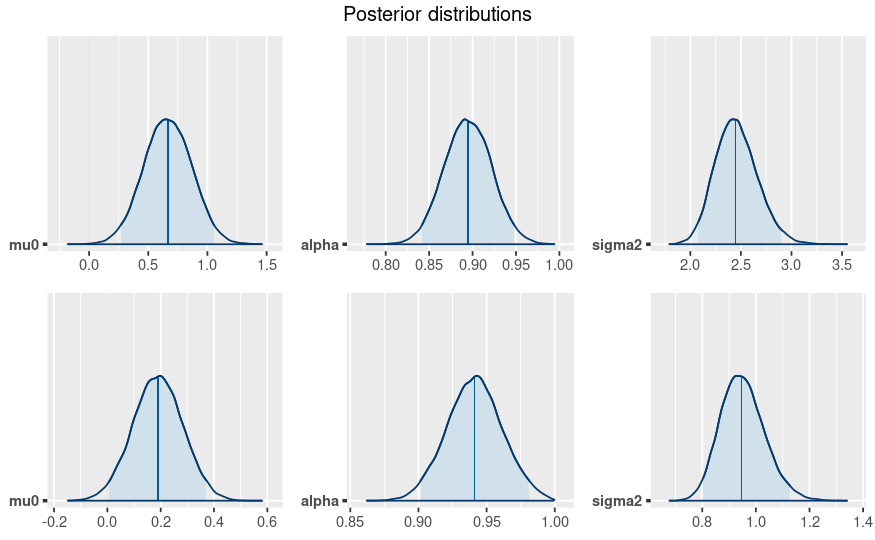
\includegraphics[width=0.8\textwidth]{images/2-AR/posteriors.png}
    \caption{Posterior distributions of the parameters for the AR(1) models. The top line corresponds to the model used for GDP, while the bottom line corresponds to the model used for CPIAUCSL.}
    \label{fig:AR1_posteriors}
\end{figure}
\begin{table}[H]
    \centering
    \begin{tabular}{c|c|c|c}
        \textbf{Model target variable } & \textbf{Parameter } & \textbf{Posterior Mean } & \textbf{95\% Credible Interval } \\
        \cline{1-4}
        GDP      & $\mu_0$    & 0.6646012 & (0.269216192, 1.0554382) \\
        GDP      & $\alpha$   & 0.8946932 & (0.842044515, 0.9481597) \\
        GDP      & $\sigma^2$ & 2.4565718 & (2.080629925, 2.8999602) \\
        CPIAUCSL & $\mu_0$    & 0.1891912 & (0.006510675, 0.3713430) \\
        CPIAUCSL & $\alpha$   & 0.9411750 & (0.901591825, 0.9812118) \\
        CPIAUCSL & $\sigma^2$ & 0.9510602 & (0.804012999, 1.1263014) \\
    \end{tabular}
    \caption{Posterior means and 95\% credible intervals for the parameters of the AR(1) models.}
    \label{tab:AR1_posteriors}
\end{table}
As seen from the posteriors, the $\alpha$ parameter is close to 1 for both GDP and CPIAUCSL. However, when using a prior for $\alpha$ over a larger range, i.e., $\alpha \sim \mathcal{U}(-2.0, 2.0)$, the estimated value of $\alpha$ did not change significantly. \\
We also examined the trace plots and autocorrelation plots and found no significant issues. \\
Lastly, we plotted the in-sample and out-of-sample predictions with 95\% credible intervals and compared them with the actual data. The results are shown in Figures \ref{fig:AR1_gdp_prediction} and \ref{fig:AR1_infl_prediction}. \\
Analyzing the out-of-sample predictions, we observe that the AR(1) model successfully captures the initial data trend. However, the model fails to anticipate the significant impact of the COVID-19 pandemic, which led to a sharp decline in GDP and a steep rise in CPIAUCSL. \\
\begin{figure}[H]
    \centering
    \begin{minipage}{0.49\textwidth}
        \centering
        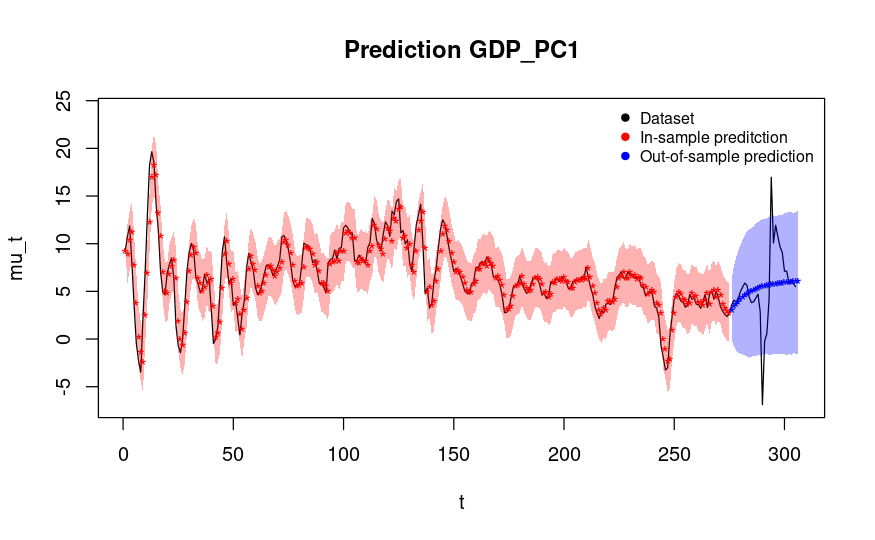
\includegraphics[width=\textwidth]{images/2-AR/gdp_prediction.png}
        \caption{In-sample and out-of-sample predictions for the GDP using the AR(1) model.}
        \label{fig:AR1_gdp_prediction}
    \end{minipage}\hfill
    \begin{minipage}{0.49\textwidth}
        \centering
        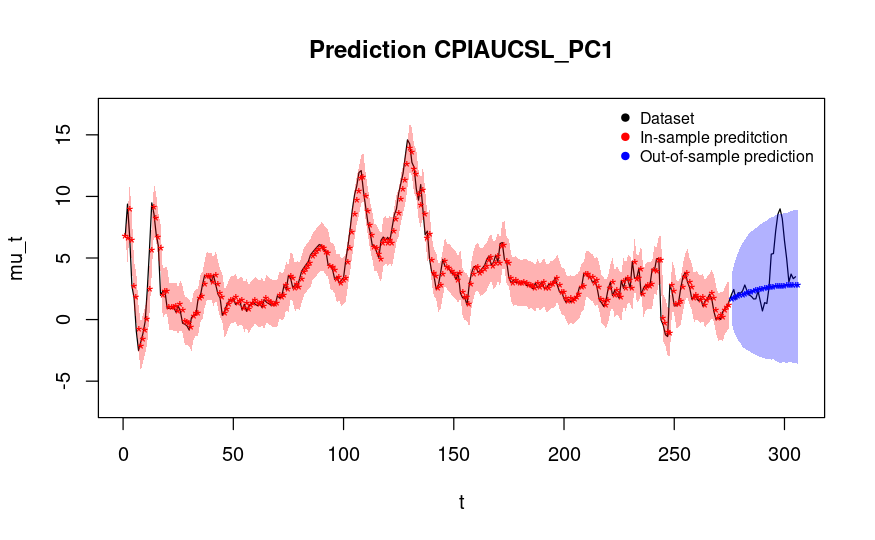
\includegraphics[width=\textwidth]{images/2-AR/infl_prediction.png}
        \caption{In-sample and out-of-sample predictions for the CPIAUCSL using the AR(1) model.}
        \label{fig:AR1_infl_prediction}
    \end{minipage}
\end{figure}
Finally, we compared the model's in-sample predictions and posterior distributions with those obtained from the AR model using the ARIMA function. Detailed comparison results are provided in the Appendix, showing no significant differences between them.